\documentclass{article}
\usepackage[T1]{fontenc}
\usepackage[utf8]{inputenc}
\usepackage{lmodern}
\usepackage[tmargin=0.75in,lmargin=0.75in,rmargin=0.75in]{geometry}
\usepackage{subcaption}
\usepackage{xcolor}
\usepackage{graphicx}
\usepackage{subcaption}


\begin{document}
\renewcommand{\baselinestretch}{1.0}
\begin{center}
\Large{\textbf{FastQC Quality Results}}
\end{center}
\section{Basic Statistics}
\begin{description}
\item[Filename:]
04{-}R1.qfilter.fastq.gz
\item[File type:]
Conventional base calls
\item[Encoding:]
Sanger / Illumina 1.9
\item[Total Sequences:]
310338
\item[Sequences flagged as poor quality:]
0
\item[Sequence length:]
50{-}150
\item[\%GC:]
40
\end{description}


\section{Summary}
\begin{tabular}{p{5cm}|c}
Parameter&Pass/Warning/Fail\\
\hline
Basic Statistics&\textcolor{green}{PASS}\\
Per base sequence quality&\textcolor{green}{PASS}\\
Per tile sequence quality&\textcolor{green}{PASS}\\
Per sequence quality scores&\textcolor{green}{PASS}\\
Per base sequence content&\textcolor{red}{FAIL}\\
Per sequence GC content&\textcolor{red}{FAIL}\\
Per base N content&\textcolor{green}{PASS}\\
Sequence Length Distribution&\textcolor{orange}{WARN}\\
Sequence Duplication Levels&\textcolor{red}{FAIL}\\
Overrepresented sequences&\textcolor{green}{PASS}\\
Adapter Content&\textcolor{green}{PASS}\\
Kmer Content&\textcolor{orange}{WARN}\\
\end{tabular}


\begin{figure}[htbp]
\centering
\begin{subfigure}{0.45\linewidth}
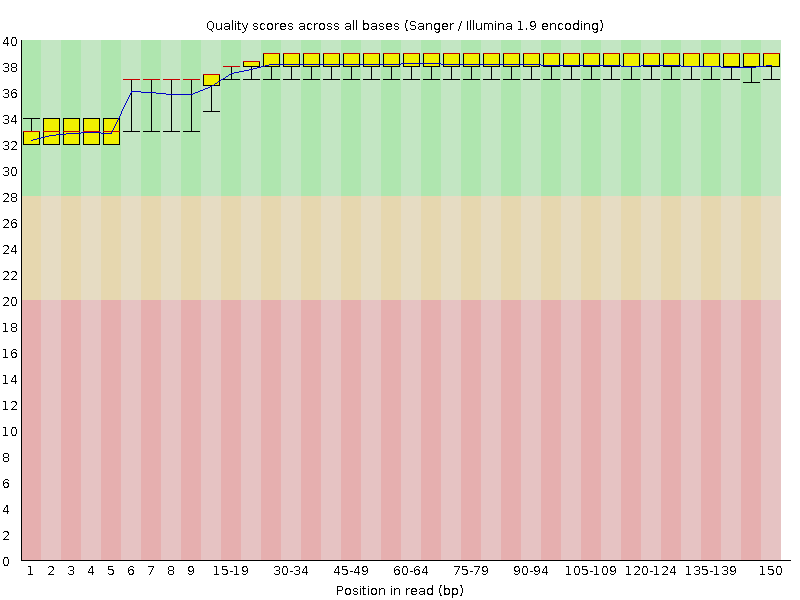
\includegraphics[width=\linewidth]{04-R1.qfilter_fastqc/Images/per_base_quality.png}
\caption{Per base sequence quality}
\end{subfigure}
\begin{subfigure}{0.45\linewidth}
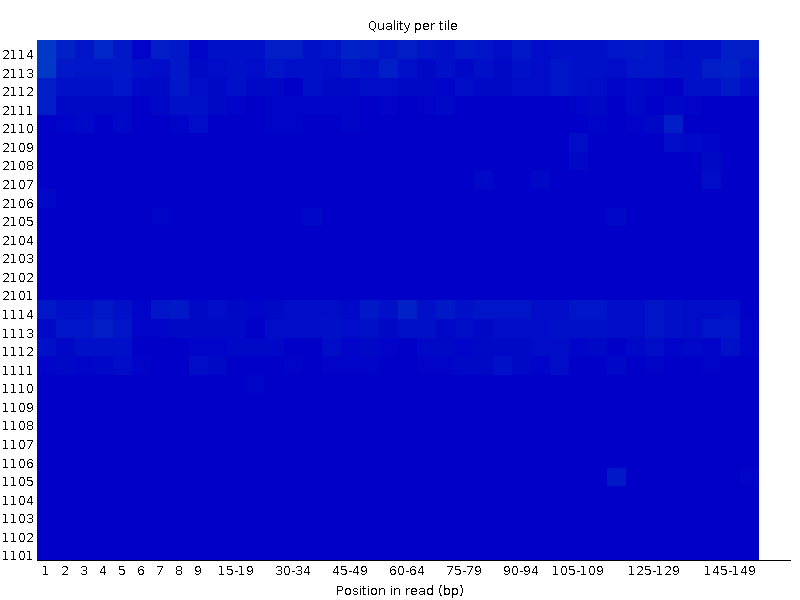
\includegraphics[width=\linewidth]{04-R1.qfilter_fastqc/Images/per_tile_quality.png}
\caption{Per tile sequence quality}
\end{subfigure}
\begin{subfigure}{0.45\linewidth}
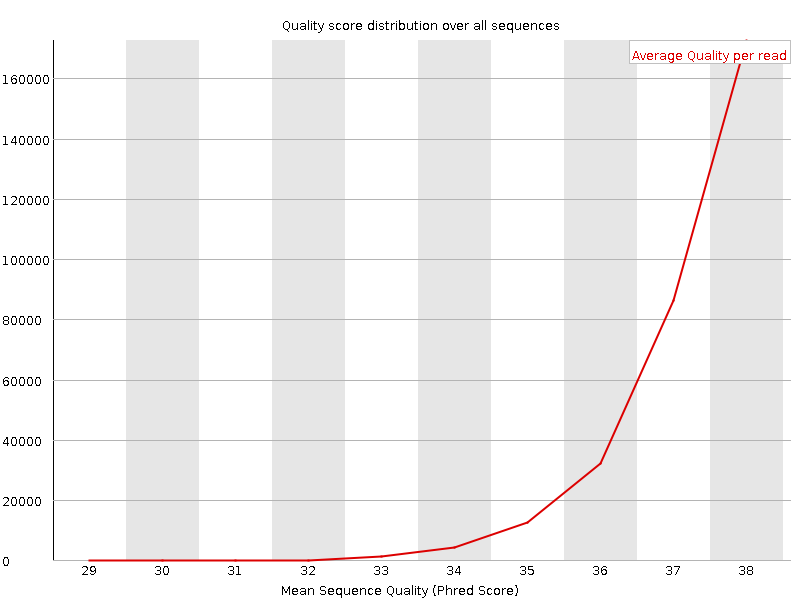
\includegraphics[width=\linewidth]{04-R1.qfilter_fastqc/Images/per_sequence_quality.png}
\caption{Per sequence quality scores}
\end{subfigure}
\begin{subfigure}{0.45\linewidth}
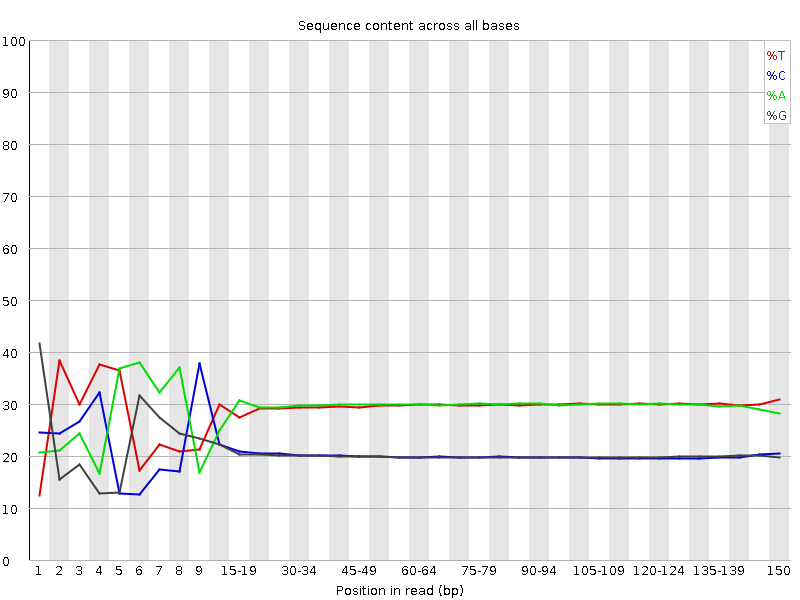
\includegraphics[width=\linewidth]{04-R1.qfilter_fastqc/Images/per_base_sequence_content.png}
\caption{Per base sequence content}
\end{subfigure}
\begin{subfigure}{0.45\linewidth}
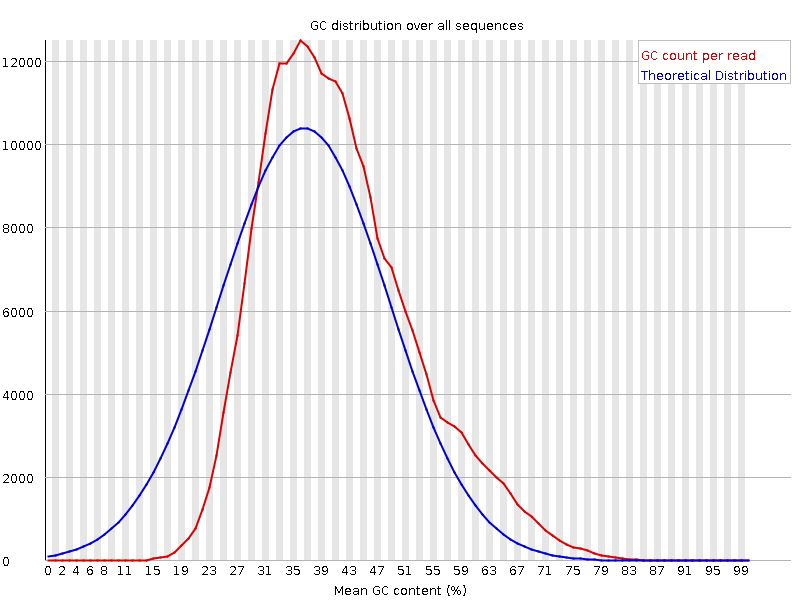
\includegraphics[width=\linewidth]{04-R1.qfilter_fastqc/Images/per_sequence_gc_content.png}
\caption{Per sequence GC content}
\end{subfigure}
\begin{subfigure}{0.45\linewidth}
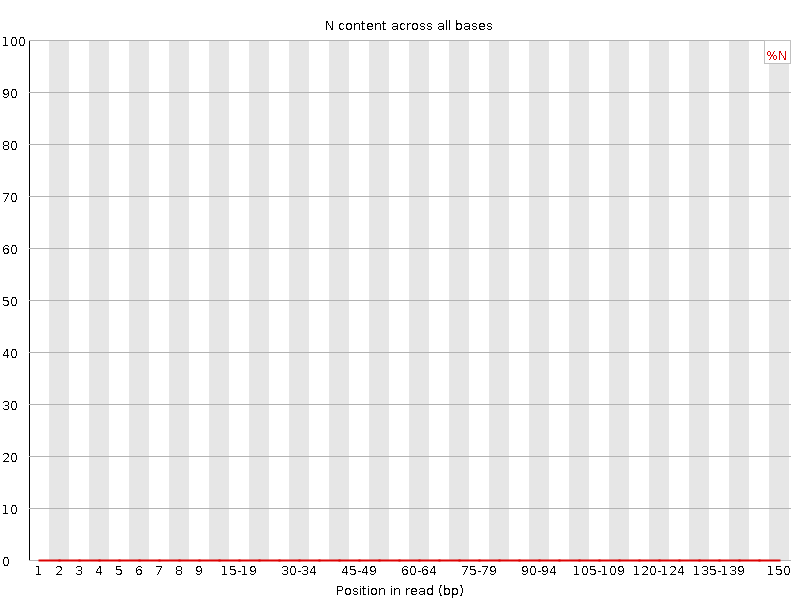
\includegraphics[width=\linewidth]{04-R1.qfilter_fastqc/Images/per_base_n_content.png}
\caption{Per base N content}
\end{subfigure}
\end{figure}




\begin{figure}[htbp]
\ContinuedFloat
\centering
\begin{subfigure}{0.45\linewidth}
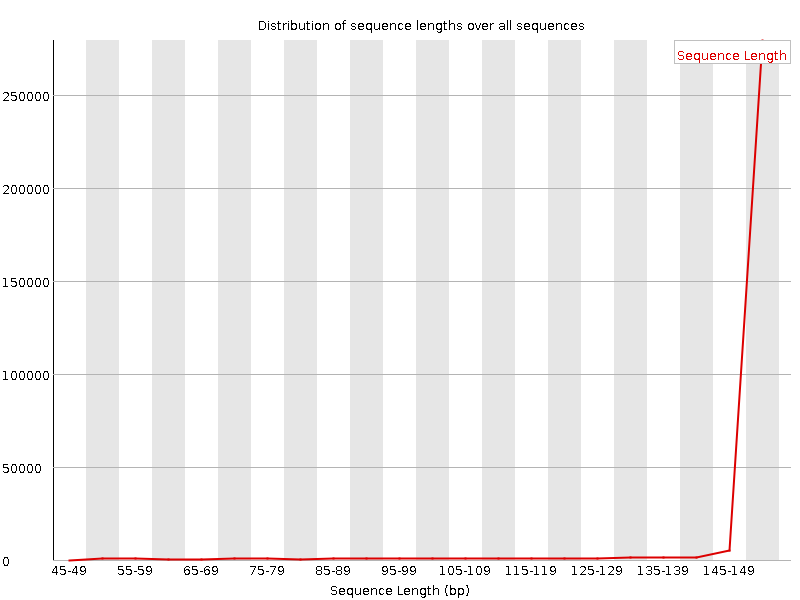
\includegraphics[width=\linewidth]{04-R1.qfilter_fastqc/Images/sequence_length_distribution.png}
\caption{Sequence Length Distribution}
\end{subfigure}
\begin{subfigure}{0.45\linewidth}
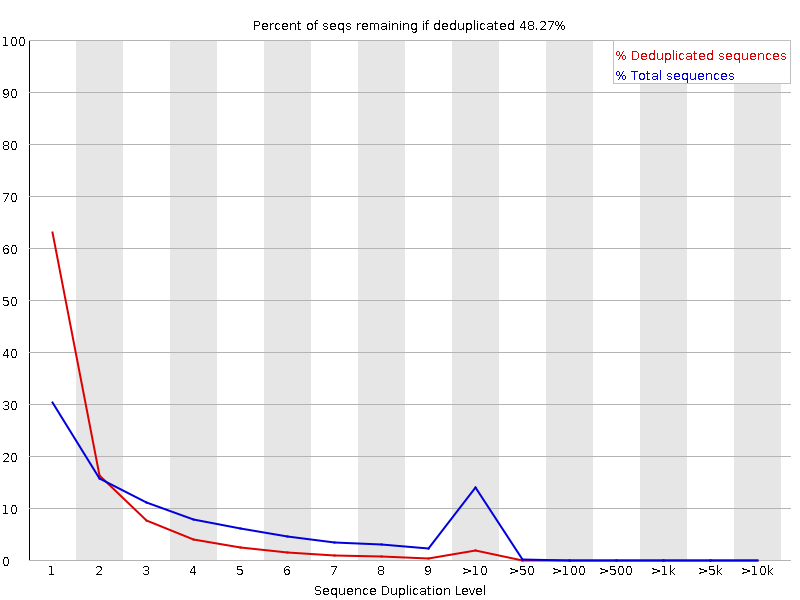
\includegraphics[width=\linewidth]{04-R1.qfilter_fastqc/Images/duplication_levels.png}
\caption{Sequence Duplication Levels}
\end{subfigure}
\begin{subfigure}{0.45\linewidth}
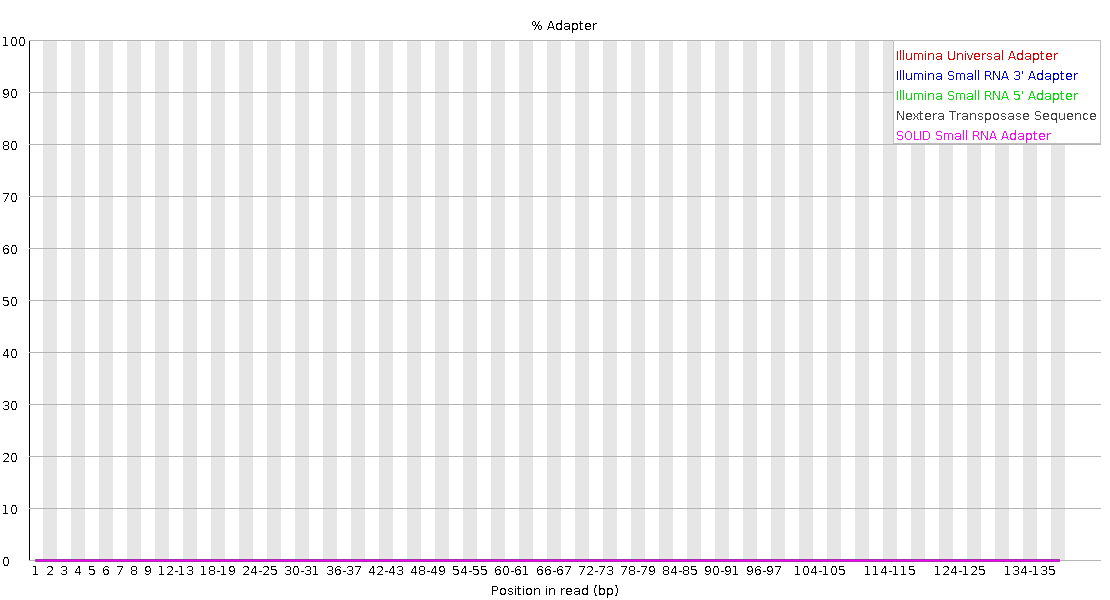
\includegraphics[width=\linewidth]{04-R1.qfilter_fastqc/Images/adapter_content.png}
\caption{Adapter content: \%s}
\end{subfigure}
\begin{subfigure}{0.45\linewidth}
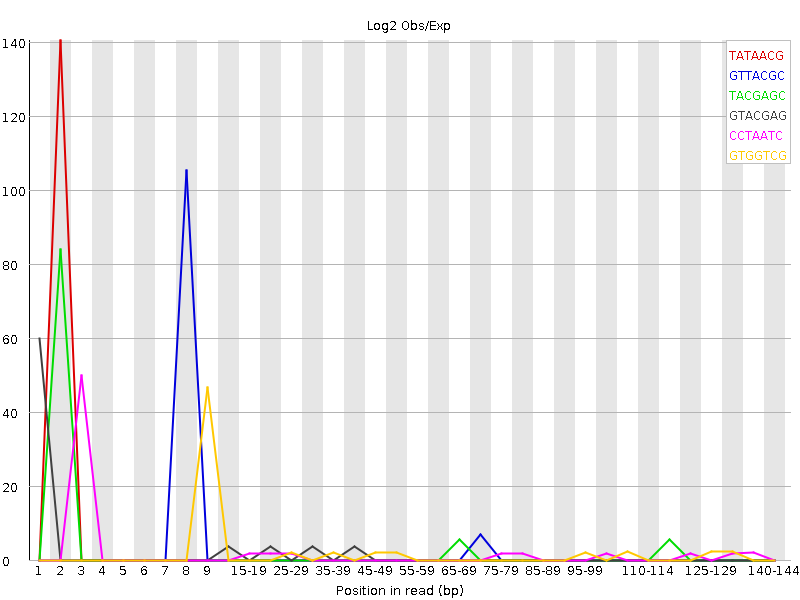
\includegraphics[width=\linewidth]{04-R1.qfilter_fastqc/Images/kmer_profiles.png}
\caption{Kmer content: \%s}
\end{subfigure}
\end{figure}


\end{document}